\documentclass{standalone}
\usepackage{graphicx}	
\usepackage{amssymb, amsmath}
\usepackage{color}
\usepackage{wasysym}

\usepackage{tikz}
\usetikzlibrary{intersections, backgrounds}
\usepackage{pgfmath}

\definecolor{light}{RGB}{220, 188, 188}
\definecolor{mid}{RGB}{185, 124, 124}
\definecolor{dark}{RGB}{143, 39, 39}
\definecolor{highlight}{RGB}{180, 31, 180}
\definecolor{gray10}{gray}{0.1}
\definecolor{gray20}{gray}{0.2}
\definecolor{gray30}{gray}{0.3}
\definecolor{gray40}{gray}{0.4}
\definecolor{gray60}{gray}{0.6}
\definecolor{gray70}{gray}{0.7}
\definecolor{gray80}{gray}{0.8}
\definecolor{gray90}{gray}{0.9}
\definecolor{gray95}{gray}{0.95}

\newcommand*{\offset}{0.025}

\begin{document}

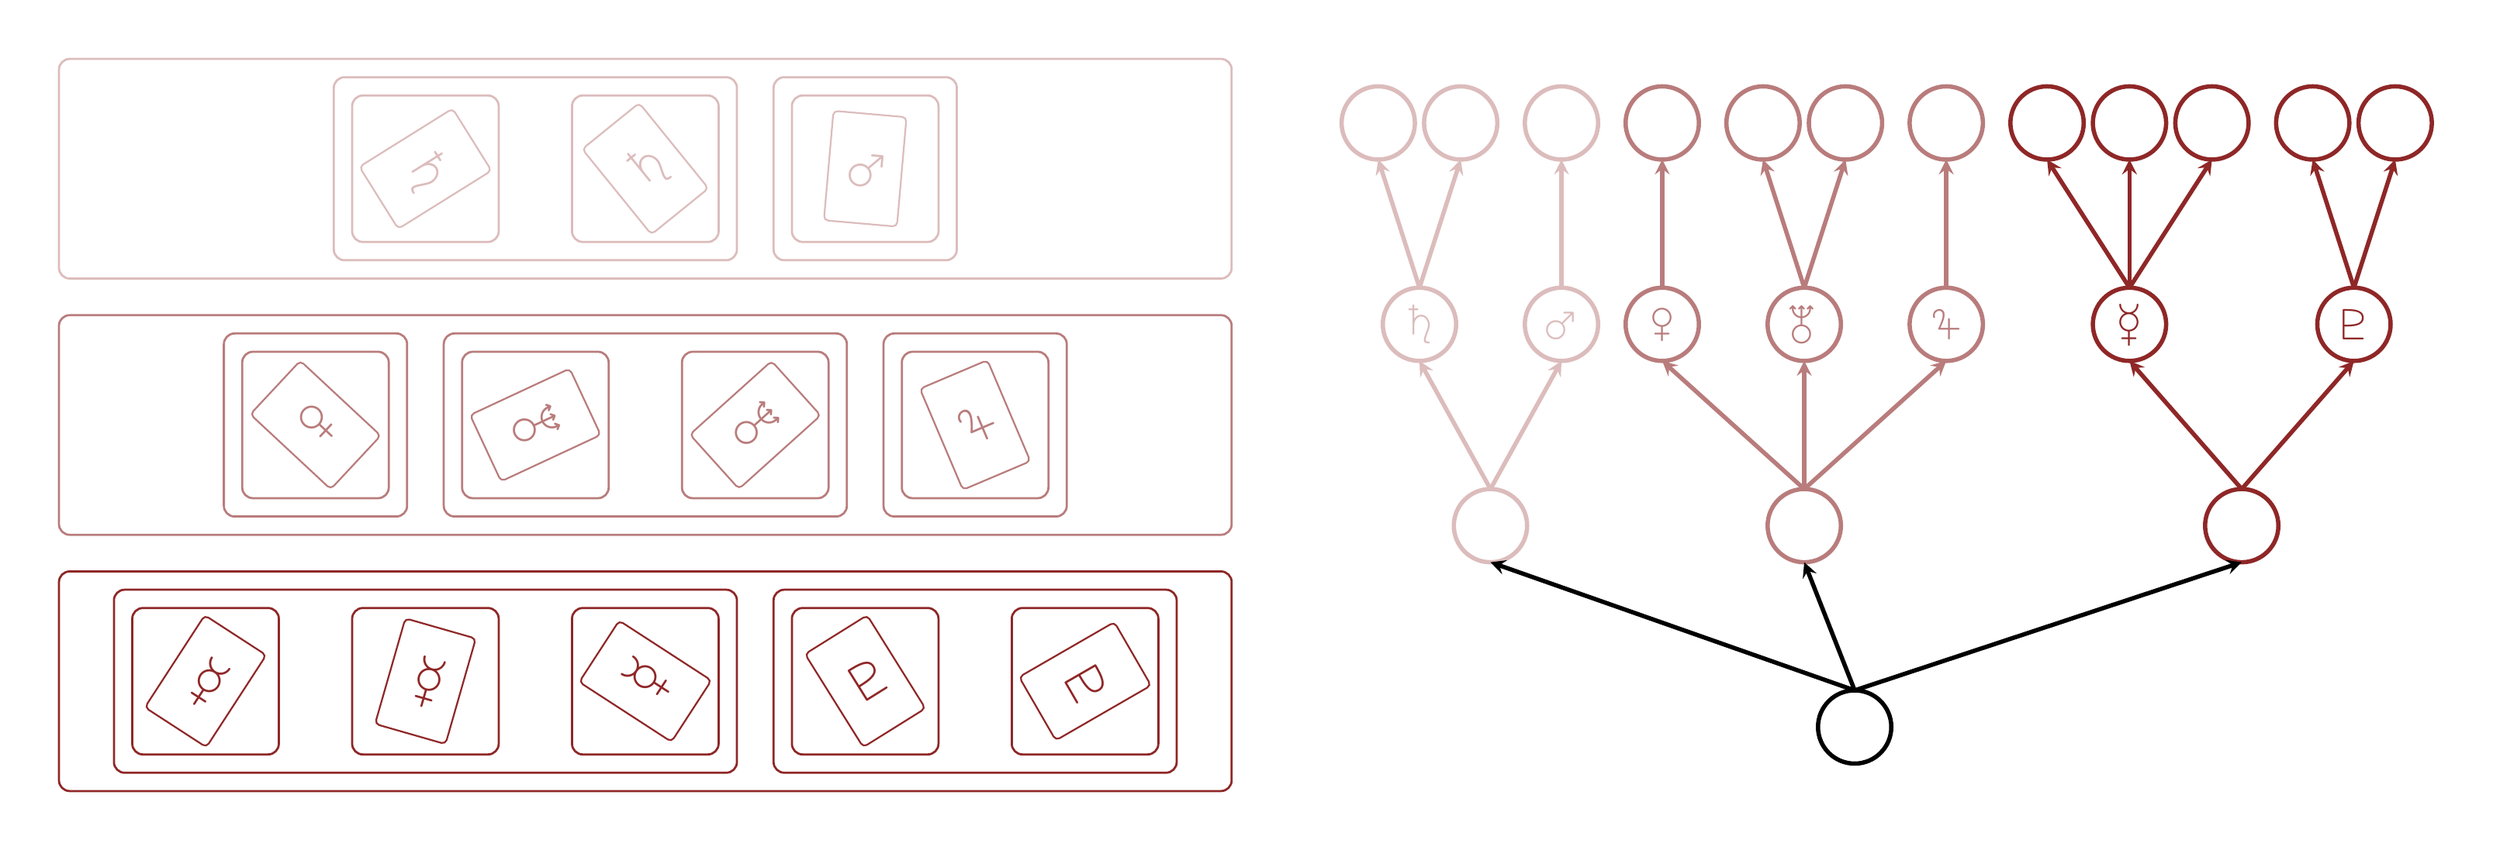
\begin{tikzpicture}[scale=0.3, thick]

\pgfmathsetmacro{\cx}{2}
\pgfmathsetmacro{\cy}{3}

\draw[white] (-34, -22) rectangle (100, 22);

\draw[light, rounded corners=5, line width=1] (-32, 14 - 6) rectangle (32, 14 + 6);
\draw[mid, rounded corners=5, line width=1] (-32, 0 - 6) rectangle (32, 0 + 6);
\draw[dark, rounded corners=5, line width=1] (-32, -14 - 6) rectangle (32, -14 + 6);

\draw[light, rounded corners=5, line width=1] (-12 - 5, 14 - 5) rectangle +(22, 10);
\draw[light, rounded corners=5, line width=1] (12 - 5, 14 - 5) rectangle +(10, 10);

\draw[light, rounded corners=5, line width=1] (-12 - 4, 14 - 4) rectangle +(8, 8);
\draw[light, rounded corners=5, line width=1] (0 - 4, 14 - 4) rectangle +(8, 8);
\draw[light, rounded corners=5, line width=1] (12 - 4, 14 - 4) rectangle +(8, 8);


\draw[mid, rounded corners=5, line width=1] (-18 - 5, 0 - 5) rectangle +(10, 10);
\draw[mid, rounded corners=5, line width=1] (-6 - 5, 0 - 5) rectangle +(22, 10);
\draw[mid, rounded corners=5, line width=1] (18 - 5, 0 - 5) rectangle +(10, 10);

\draw[mid, rounded corners=5, line width=1] (-18 - 4, 0 - 4) rectangle +(8, 8);
\draw[mid, rounded corners=5, line width=1] (-6 - 4, 0 - 4) rectangle +(8, 8);
\draw[mid, rounded corners=5, line width=1] (6 - 4, 0 - 4) rectangle +(8, 8);
\draw[mid, rounded corners=5, line width=1] (18 - 4, 0 - 4) rectangle +(8, 8);

\draw[dark, rounded corners=5, line width=1] (-24 - 5, -14 - 5) rectangle +(34, 10);
\draw[dark, rounded corners=5, line width=1] (12 - 5, -14 - 5) rectangle +(22, 10);

\draw[dark, rounded corners=5, line width=1] (-24 - 4, -14 - 4) rectangle +(8, 8);
\draw[dark, rounded corners=5, line width=1] (-12 - 4, -14 - 4) rectangle +(8, 8);
\draw[dark, rounded corners=5, line width=1] (0 - 4, -14 - 4) rectangle +(8, 8);
\draw[dark, rounded corners=5, line width=1] (12 - 4, -14 - 4) rectangle +(8, 8);
\draw[dark, rounded corners=5, line width=1] (24 - 4, -14 - 4) rectangle +(8, 8);

% Row One
\pgfmathsetmacro{\phi}{-58}
\pgfmathsetmacro{\x}{-12}
\pgfmathsetmacro{\y}{14}
\begin{scope}[shift={(\x, \y)}, rotate={\phi}]
  \filldraw[fill=white, draw=light, rounded corners=2] (0 - \cx, 0 - \cy) rectangle (0 + \cx, 0 + \cy);
  \node[light, rotate={\phi}] at (0.17, 0) { $\Huge \saturn$ }; 
\end{scope}

\pgfmathsetmacro{\phi}{39}
\pgfmathsetmacro{\x}{0}
\pgfmathsetmacro{\y}{14}
\begin{scope}[shift={(\x, \y)}, rotate={\phi}]
  \filldraw[fill=white, draw=light, rounded corners=2] (0 - \cx, 0 - \cy) rectangle (0 + \cx, 0 + \cy);
  \node[light, rotate={\phi}] at (0.17, 0) { $\Huge \saturn$ }; 
\end{scope}

\pgfmathsetmacro{\phi}{-5}
\pgfmathsetmacro{\x}{12}
\pgfmathsetmacro{\y}{14}
\begin{scope}[shift={(\x, \y)}, rotate={\phi}]
  \filldraw[fill=white, draw=light, rounded corners=2] (0 - \cx, 0 - \cy) rectangle (0 + \cx, 0 + \cy);
  \node[light, rotate={\phi}] at (0.17, 0) { $\Huge \mars$ }; 
\end{scope}

% Row Two
\pgfmathsetmacro{\phi}{47}
\pgfmathsetmacro{\x}{-18}
\pgfmathsetmacro{\y}{0}
\begin{scope}[shift={(\x, \y)}, rotate={\phi}]
  \filldraw[fill=white, draw=mid, rounded corners=2] (0 - \cx, 0 - \cy) rectangle (0 + \cx, 0 + \cy);
  \node[mid, rotate={\phi}] at (0.17, 0) { $\Huge \venus$ }; 
\end{scope}

\pgfmathsetmacro{\phi}{-65}
\pgfmathsetmacro{\x}{-6}
\pgfmathsetmacro{\y}{0}
\begin{scope}[shift={(\x, \y)}, rotate={\phi}]
  \filldraw[fill=white, draw=mid, rounded corners=2] (0 - \cx, 0 - \cy) rectangle (0 + \cx, 0 + \cy);
  \node[mid, rotate={\phi}] at (0.17, 0) { $\Huge \neptune$ }; 
\end{scope}

\pgfmathsetmacro{\phi}{-48}
\pgfmathsetmacro{\x}{6}
\pgfmathsetmacro{\y}{0}
\begin{scope}[shift={(\x, \y)}, rotate={\phi}]
  \filldraw[fill=white, draw=mid, rounded corners=2] (0 - \cx, 0 - \cy) rectangle (0 + \cx, 0 + \cy);
  \node[mid, rotate={\phi}] at (0.17, 0) { $\Huge \neptune$ }; 
\end{scope}

\pgfmathsetmacro{\phi}{23}
\pgfmathsetmacro{\x}{18}
\pgfmathsetmacro{\y}{0}
\begin{scope}[shift={(\x, \y)}, rotate={\phi}]
  \filldraw[fill=white, draw=mid, rounded corners=2] (0 - \cx, 0 - \cy) rectangle (0 + \cx, 0 + \cy);
  \node[mid, rotate={\phi}] at (0.17, 0) { $\Huge \jupiter$ }; 
\end{scope}

% Row Three
\pgfmathsetmacro{\phi}{-33}
\pgfmathsetmacro{\x}{-24}
\pgfmathsetmacro{\y}{-14}
\begin{scope}[shift={(\x, \y)}, rotate={\phi}]
  \filldraw[fill=white, draw=dark, rounded corners=2] (0 - \cx, 0 - \cy) rectangle (0 + \cx, 0 + \cy);
  \node[dark, rotate={\phi}] at (0.17, 0) { $\Huge \mercury$ }; 
\end{scope}

\pgfmathsetmacro{\phi}{-16}
\pgfmathsetmacro{\x}{-12}
\pgfmathsetmacro{\y}{-14}
\begin{scope}[shift={(\x, \y)}, rotate={\phi}]
  \filldraw[fill=white, draw=dark, rounded corners=2] (0 - \cx, 0 - \cy) rectangle (0 + \cx, 0 + \cy);
  \node[dark, rotate={\phi}] at (0.17, 0) { $\Huge \mercury$ }; 
\end{scope}

\pgfmathsetmacro{\phi}{57}
\pgfmathsetmacro{\x}{0}
\pgfmathsetmacro{\y}{-14}
\begin{scope}[shift={(\x, \y)}, rotate={\phi}]
  \filldraw[fill=white, draw=dark, rounded corners=2] (0 - \cx, 0 - \cy) rectangle (0 + \cx, 0 + \cy);
  \node[dark, rotate={\phi}] at (0.17, 0) { $\Huge \mercury$ }; 
\end{scope}

\pgfmathsetmacro{\phi}{32}
\pgfmathsetmacro{\x}{12}
\pgfmathsetmacro{\y}{-14}
\begin{scope}[shift={(\x, \y)}, rotate={\phi}]
  \filldraw[fill=white, draw=dark, rounded corners=2] (0 - \cx, 0 - \cy) rectangle (0 + \cx, 0 + \cy);
  \node[dark, rotate={\phi}] at (0.17, 0) { $\Huge \pluto$ }; 
\end{scope}

\pgfmathsetmacro{\phi}{-60}
\pgfmathsetmacro{\x}{24}
\pgfmathsetmacro{\y}{-14}
\begin{scope}[shift={(\x, \y)}, rotate={\phi}]
  \filldraw[fill=white, draw=dark, rounded corners=2] (0 - \cx, 0 - \cy) rectangle (0 + \cx, 0 + \cy);
  \node[dark, rotate={\phi}] at (0.17, 0) { $\Huge \pluto$ }; 
\end{scope}

\pgfmathsetmacro{\r}{2}

% Light
\filldraw[fill=white, draw=light, line width=2] (40, 16.5) circle (\r);
\filldraw[fill=white, draw=light, line width=2] (44.5, 16.5) circle (\r);

\draw[->, >=stealth, color=light, line width=2] (42.25, 5.5 + \r) -- (40, 16.5 - \r);
\draw[->, >=stealth, color=light, line width=2] (42.25, 5.5 + \r) -- (44.5, 16.5 - \r);

\filldraw[fill=white, draw=light, line width=2] (42.25, 5.5) circle (\r)
node[color=light] { $\huge \saturn$ };

\filldraw[fill=white, draw=light, line width=2] (50, 16.5) circle (\r);

\draw[->, >=stealth, color=light, line width=2] (50, 5.5 + \r) -- (50, 16.5 - \r);

\filldraw[fill=white, draw=light, line width=2] (50, 5.5) circle (\r)
node[color=light] { $\huge \mars$ };

\draw[->, >=stealth, color=light, line width=2] (46.125, -5.5 + \r) -- (42.25, 5.5 - \r);
\draw[->, >=stealth, color=light, line width=2] (46.125, -5.5 + \r) -- (50, 5.5 - \r);

\filldraw[fill=white, draw=light, line width=2] (46.125, -5.5) circle (\r);


% Mid
\filldraw[fill=white, draw=mid, line width=2] (55.5, 16.5) circle (\r);

\draw[->, >=stealth, color=mid, line width=2] (55.5, 5.5 + \r) -- (55.5, 16.5 - \r);

\filldraw[fill=white, draw=mid, line width=2] (55.5, 5.5) circle (\r)
node[color=mid] { $\huge \venus$ };

\filldraw[fill=white, draw=mid, line width=2] (61, 16.5) circle (\r);
\filldraw[fill=white, draw=mid, line width=2] (65.5, 16.5) circle (\r);

\draw[->, >=stealth, color=mid, line width=2] (63.25, 5.5 + \r) -- (61, 16.5 - \r);
\draw[->, >=stealth, color=mid, line width=2] (63.25, 5.5 + \r) -- (65.5, 16.5 - \r);

\filldraw[fill=white, draw=mid, line width=2] (63.25, 5.5) circle (\r)
node[color=mid] { $\huge \neptune$ };

\filldraw[fill=white, draw=mid, line width=2] (71, 16.5) circle (\r);

\draw[->, >=stealth, color=mid, line width=2] (71, 5.5 + \r) -- (71, 16.5 - \r);

\filldraw[fill=white, draw=mid, line width=2] (71, 5.5) circle (\r)
node[color=mid] { $\huge \jupiter$ };

\draw[->, >=stealth, color=mid, line width=2] (63.25, -5.5 + \r) -- (55.5, 5.5 - \r);
\draw[->, >=stealth, color=mid, line width=2] (63.25, -5.5 + \r) -- (63.25, 5.5 - \r);
\draw[->, >=stealth, color=mid, line width=2] (63.25, -5.5 + \r) -- (71, 5.5 - \r);

\filldraw[fill=white, draw=mid, line width=2] (63.25, -5.5) circle (\r);


% Dark
\filldraw[fill=white, draw=dark, line width=2] (76.5, 16.5) circle (\r);
\filldraw[fill=white, draw=dark, line width=2] (81, 16.5) circle (\r);
\filldraw[fill=white, draw=dark, line width=2] (85.5, 16.5) circle (\r);

\draw[->, >=stealth, color=dark, line width=2] (81, 5.5 + \r) -- (76.5, 16.5 - \r);
\draw[->, >=stealth, color=dark, line width=2] (81, 5.5 + \r) -- (81, 16.5 - \r);
\draw[->, >=stealth, color=dark, line width=2] (81, 5.5 + \r) -- (85.5, 16.5 - \r);

\filldraw[fill=white, draw=dark, line width=2] (81, 5.5) circle (\r)
node[color=dark] { $\huge \mercury$ };

\filldraw[fill=white, draw=dark, line width=2] (91, 16.5) circle (\r);
\filldraw[fill=white, draw=dark, line width=2] (95.5, 16.5) circle (\r);

\draw[->, >=stealth, color=dark, line width=2] (93.25, 5.5 + \r) -- (91, 16.5 - \r);
\draw[->, >=stealth, color=dark, line width=2] (93.25, 5.5 + \r) -- (95.5, 16.5 - \r);

\filldraw[fill=white, draw=dark, line width=2] (93.25, 5.5) circle (\r)
node[color=dark] { $\huge \pluto$ };

\draw[->, >=stealth, color=dark, line width=2] (87.125, -5.5 + \r) -- (81, 5.5 - \r);
\draw[->, >=stealth, color=dark, line width=2] (87.125, -5.5 + \r) -- (93.25, 5.5 - \r);

\filldraw[fill=white, draw=dark, line width=2] (87.125, -5.5) circle (\r);

\draw[->, >=stealth, color=black, line width=2] (66, -16.5 + \r) -- (46.125, -5.5 - \r);
\draw[->, >=stealth, color=black, line width=2] (66, -16.5 + \r) -- (63.25, -5.5 - \r);
\draw[->, >=stealth, color=black, line width=2] (66, -16.5 + \r) -- (87.125, -5.5 - \r);

\filldraw[fill=white, draw=black, line width=2] (66, -16.5) circle (\r);


\end{tikzpicture}

\end{document}  